\graphicspath{{./images/}}

\chapter{Einführung und Ziele}

\section{Business Case}

Die Applikation MEON dient der Registration neuer händler für den mobilen Bezahldienst Twint. 

\begin{center}
	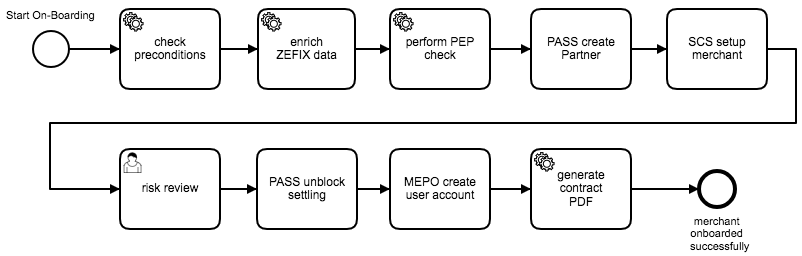
\includegraphics[scale=0.55]{meon-workflow.png}
\end{center}


\section{Aufgabenstellung}

Die die bestehende Merchant Onboarding Applikation soll eine neue Architektur entwickelt werden welche Continuous Deployment erlaubt.

\section{Qualitätsziele}

\section{Stakeholder}

\begin{table}[H]
	\centering
	\caption{Stakeholder}
	\begin{tabular}{ | p{2cm} | p{14cm} | }
		\toprule
		{\textbf{Name}} & {\textbf{Beschreibung}} \\
		\midrule
		Business & Repräsentiert die Geschäftstätigkeit der Firma.\\ \hline
		Kunde & Benutzer der Webapplikation. \\ \hline
		Support-Kunde & Support welcher den Kunden bei Problemen unterstützt. \\ \hline
		Legal &  Verantwortlich für die Richtigkeit der Vertragsabschlüsse. \\ \hline
		Risk & Sorgt für die Überprüfung der Personen und der Geschäftstätigkeiten. \\ \hline
		Communications & Abteilung für den Vertrieb, Werbung, Design. \\ \hline
		Betrieb & Betreibt die Webapplikation auf der Infrastruktur der SIX \\ \hline
		Change Management & Genehmigt Änderungen an der Applikation. \\ \hline
		Entwickler & Setzt die Anforderungen der einzelnen Stakeholder um. \\ 
		\bottomrule
	\end{tabular}
\end{table}